\documentclass[10pt,twocolumn]{article}
\usepackage[a4paper,margin=1.45cm,top=1.2cm,bottom=1.3cm]{geometry}
\usepackage[T1]{fontenc}
\usepackage{lmodern}
\usepackage{microtype}
\usepackage{amsmath}
\usepackage{booktabs}
\usepackage{graphicx}
\usepackage{caption}
\usepackage{titlesec}
\usepackage[hidelinks]{hyperref}
\captionsetup{font=small,labelfont=bf,skip=3pt}
\titlespacing*{\section}{0pt}{7pt}{3pt}
\titlespacing*{\subsection}{0pt}{5pt}{2pt}
\titleformat*{\section}{\normalsize\bfseries}
\titleformat*{\subsection}{\small\bfseries}
\setlength{\columnsep}{0.65cm}
\setlength{\parskip}{0pt}
\setlength{\abovecaptionskip}{3pt}
\renewcommand{\arraystretch}{1.08}

\title{\vspace{-1.1cm}\large\bfseries Quantum sampling for a long/short stock split:\\an honest benchmark of QAOA variants on 12--29 qubits}
\author{\normalsize Team ZollerQu (Oussema-t, Tushar Pandey)\\\small Qollab $\times$ IonQ Hackathon, 9--11 October 2026 \quad---\quad This effort is supported by Qollab \& IonQ.}
\date{}

\begin{document}
\maketitle
\vspace{-0.9cm}

\begin{abstract}\noindent
We encode the choice of a low-risk long/short (or buy/skip) stock portfolio as an Ising problem with one qubit per asset, solve it exactly and with classical heuristics at 12 assets, and benchmark seven quantum circuit families (linear-ramp QAOA, free-angle QAOA with five optimisers, CVaR, multi-angle, counterdiabatic, two imaginary-time methods and a constraint-preserving XY mixer) on an exact statevector simulator against the same answer key. Tuned circuits sample the optimal portfolio 30--236 times more often than uniform guessing and, in long/short mode, return it as their single most likely answer; they do not beat greedy descent or simulated annealing. We report a sign error in the linear-ramp recipe as commonly written, measure the all-to-all connectivity advantage (66 vs.\ 285 two-qubit gates per layer at 12 qubits, 244 vs.\ 1\,576 at 29), and show that angles tuned at 12 qubits transfer to 16 and 20. All optimised portfolios reduced out-of-sample risk; none beat the market's return. No quantum advantage is claimed; no hardware run is reported here.
\end{abstract}

\section{Problem and data}
Each asset $i$ gets a spin $s_i\in\{+1,-1\}$. Mode~A (long/short): $+1$ = buy, $-1$ = short, weights $s_i/n$. Mode~B (buy/skip): $x_i=(1+s_i)/2\in\{0,1\}$, weight $x_i/n$, the rest in cash. With training-window mean weekly log returns $\mu$ and sample covariance $C$, the score to minimise is
\begin{equation}
J = \frac{w^{\mathsf T} C\, w}{V_{\mathrm{ref}}} - \eta\,\frac{\mu^{\mathsf T} w}{\sigma_{\mathrm{ref}}},\qquad V_{\mathrm{ref}}=\overline{\operatorname{diag} C},
\end{equation}
with $\eta\in\{0.25,0.5,1,2\}$ ($\eta=1$ default) and an optional balance constraint (equal numbers on each side). $J$ is an Ising energy $\sum_{i<j}J_{ij}s_is_j+\sum_i h_i s_i+c$ exactly (verified to $10^{-16}$); thinning the 29-asset couplings to the strongest 60\,\% by $|\rho_{ij}|$ gives a surrogate within 0.013 of the true score (rank correlation 0.975).

\textbf{Data.} Kaggle ``Huge Stock Market Dataset'' (CC0): 29 named US assets in 10 groups (tech, gold \& silver, energy, banks, bonds, healthcare, staples, utilities, real estate, copper) plus SPY as a reference, weekly closes 2006-05-26 to 2017-11-10 (599 weeks). Chronological split: 418 training weeks (to 2014-05-30, containing the 2008 crash) and 180 held-out weeks. Nothing was tuned on the test weeks. The 12-asset instance is one asset per group in a fixed round-robin: AAPL, GLD, XOM, JPM, TLT, JNJ, PG, XLU, VNQ, FCX, MSFT, SLV. Bonds are the only group negatively correlated with the rest (mean $\rho\approx-0.22$; TLT--XLK $-0.45$); gold is near zero.

\section{Methods}
\textbf{Answer key and classical baselines.} At 12 assets all $2^{12}=4\,096$ portfolios are enumerated (one optimum per setting). Baselines, written in NumPy: uniform random sampling, greedy single-flip/swap descent and simulated annealing, three seeds each; balance is a verified penalty $\lambda(\sum_i s_i)^2$ at 12 assets and a hard constraint at 29.

\textbf{Circuit.} $H^{\otimes n}$, then per layer $k$: $R_{zz}(2\gamma_k J_{ij}/\text{scale})$ on every kept link, $R_z(2\gamma_k h_i/\text{scale})$ on every asset, $R_x(2\beta_k)$ on every qubit, scale $=\max(|J|,|h|)$. Linear-ramp QAOA (LR-QAOA)~\cite{lrqaoa} uses $\gamma_k=\tfrac{k}{p}\Delta\gamma$, $\beta_k=(1-\tfrac{k-1}{p})\Delta\beta$ and was grid-tuned ($15\times20$ points, $p=1..5$) by lowest expected energy, never by the optimum's probability. Free-angle QAOA ($2p$ angles) was tuned by COBYLA, Nelder--Mead, Powell, L-BFGS-B and our own SPSA from the same five starts with a cap of $200p$ circuit evaluations. Extras at the same budget: CVaR objective ($\alpha=0.1,0.25$), multi-angle ($3p$), first-order counterdiabatic $R_y$ layer (DC-QAOA, cf.~\cite{kipu}), VarQITE angle training (McLachlan), varQITE with the Pauli-term update rule of IonQ/ORNL~\cite{varqite} (ansatz A: $R_y$+CX per link; ansatz B: $R_{zz}$ per link + $R_x$ layer; implemented from the description, no code reused), and an XY mixer with a Dicke start for the balance constraint. An independent NumPy statevector simulator (1.7\,ms per $p=2$ circuit) agrees with Qiskit~2.5.2 \texttt{Statevector} to $3\times10^{-16}$. The full run (118 unit tests) took 121\,s on 8 cores.

\textbf{Sign of the ramp.} With the mixer $R_x(+2\beta)$, lowering the energy requires $\gamma$ and $\beta$ of \emph{opposite} sign. The recipe as commonly written ($\Delta\gamma=0.6,\Delta\beta=0.3$) drives the state towards the \emph{highest} energies: quality 0.45 at $p=5$ against 0.81 for uniform sampling (mode~A). All ramps below have $\Delta\beta<0$.

\section{Results (12 qubits, $\eta=1$, exact statevector)}
Metrics: $P_{\mathrm{opt}}$ = probability that one shot is the optimal portfolio (uniform: $1/4096=0.00024$); quality $=(E_{\max}-\langle E\rangle)/(E_{\max}-E_{\min})$ of the sampled distribution.

\begin{table}[h]\centering\footnotesize\setlength{\tabcolsep}{3.5pt}
\caption{Main benchmark. Classical rows give the hit rate of the optimum per try (random: 1\,000 tries; greedy and annealing: 30 restarts, three seeds).}
\begin{tabular}{@{}lcccc@{}}\toprule
 & \multicolumn{2}{c}{Mode A} & \multicolumn{2}{c}{Mode B}\\
\cmidrule(lr){2-3}\cmidrule(lr){4-5}
Method & $P_{\mathrm{opt}}$ & quality & $P_{\mathrm{opt}}$ & quality\\\midrule
$p=0$ control (uniform) & 0.0002 & 0.807 & 0.0002 & 0.714\\
LR-QAOA, best $p$ (5 / 4) & \textbf{0.0073} & 0.950 & \textbf{0.0207} & 0.973\\
free-angle QAOA, best $p$ (3 / 2) & 0.0042 & 0.935 & 0.0122 & 0.976\\
CVaR $\alpha{=}0.1$, $p=3$ & 0.0066 & 0.918 & \textbf{0.0577} & 0.948\\
multi-angle, $p=3$ & 0.0054 & 0.945 & 0.0057 & 0.987\\
counterdiabatic, $p=3$ & 0.0067 & 0.938 & 0.0000 & 0.985\\
VarQITE (McLachlan), $p=3$ & 0.0042 & 0.935 & 0.0258 & 0.978\\
varQITE Pauli-update~\cite{varqite} & ${<}10^{-5}$ & 0.880 & ${<}10^{-5}$ & 0.871\\\midrule
random guessing (per try) & 0.000 & -- & 0.000 & --\\
greedy descent (per try) & 0.067 & -- & 1.000 & --\\
simulated annealing (per try) & 0.256 & -- & 1.000 & --\\\bottomrule
\end{tabular}
\end{table}

\begin{figure*}[t]\centering
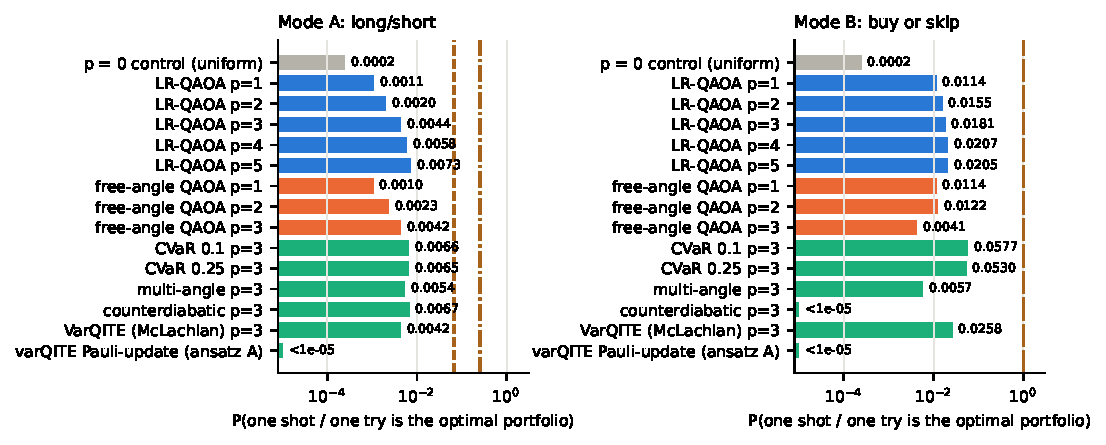
\includegraphics[width=\textwidth]{figures/ladder.pdf}
\caption{Every method on one scale: probability that a single shot (or classical try) is the optimal portfolio, log axis. Grey: uniform control; blue: LR-QAOA; orange: free-angle QAOA; green: the extras. Brown lines: classical hit rate per try, dotted = greedy (0.07 in A, 1.00 in B), dash-dot = simulated annealing (0.26 in A, 1.00 in B).}
\label{fig:ladder}
\end{figure*}

Tuned circuits beat uniform sampling by $30\times$ (A) and $85\times$ (B); the CVaR objective reaches $236\times$ in mode~B at the price of a lower mean quality. In 1\,000 shots the optimum appears at least once with probability 0.999 (A) and 1.000 (B). In mode~A the circuit's single most likely portfolio \emph{is} the optimum (rank 1 of 4\,096; long AAPL, MSFT, GLD, SLV, JPM, TLT, PG, XLU; short XOM, JNJ, VNQ, FCX; Fig.~\ref{fig:cut}); in mode~B it is ``buy TLT only'', one asset from the optimum ``buy AAPL+TLT'' (rank 6). No circuit approaches greedy or annealing, which hit the optimum in most tries: on this problem the circuit is a better-than-random sampler, not a better optimiser. The optimiser matters less than the start: from the tuned ramp all five reach about the same quality (mean over starts 0.86--0.97), random starts often stall; L-BFGS-B needs the fewest evaluations (24--98). The counterdiabatic layer in mode~B concentrates on near-optimal states but never on the optimum. varQITE learns slowly at the published learning rates; its IonQ-native ansatz~B is a stationary point at $\theta=0$ (all parameter-shift derivatives vanish) and needs a random start. Exact imaginary time on a diagonal cost is classical Boltzmann sampling; as a reference it overtakes the best LR-QAOA at $\tau=80$ (A) / 160 (B).

\begin{figure}[t]\centering
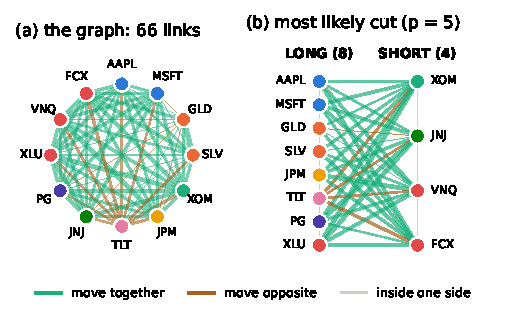
\includegraphics[width=\columnwidth]{figures/cut.pdf}
\caption{Mode A, 12 assets. (a) Training correlations: teal = move together, brown = move opposite, width $\propto|\rho|$. (b) The most likely LR-QAOA portfolio: 27 of 52 ``together'' links are cut (hedged), 5 of 14 ``opposite'' links.}
\label{fig:cut}
\end{figure}

\textbf{Balance.} The penalty coupling $2\lambda$ is $12\times$ (A) / $5\times$ (B) the largest objective term, so penalised circuits mostly learn the constraint. At $p=2$ the probability of the best \emph{balanced} portfolio per shot is 0.0011 with the penalty (97\,\% balanced shots), 0.0019 (A) / 0.0009 (B) with post-selection of the unconstrained circuit (30\,\% / 1\,\% balanced), and \textbf{0.0192} (A) / \textbf{0.0068} (B) with the XY mixer (100\,\% balanced, 12 XX+YY gates per layer; Dicke preparation not gate-optimised).

\textbf{Gate counts and transfer.} One layer needs 66 two-qubit gates (depth 15) at 12 qubits and 244 (depth 29) at 29 qubits on all-to-all connectivity, where $R_{zz}$ is native on IonQ Forte; routed on a heavy-hex grid (Qiskit transpiler, level 1, five seeds) the same layers need 285 and 1\,576 (4.3$\times$ and 6.5$\times$). The 29-qubit circuits were built and counted only. The ramp tuned at 12 assets keeps its quality at 16 (0.905 vs.\ 0.910 re-tuned) and 20 assets (0.919; 0.882 when thinned to 60\,\%), which justifies using it untuned at 29.

\textbf{Out-of-sample finance (Task 3, classical optimum).} Over the 180 held-out weeks, all 32 settings (2 modes $\times$ 4 $\eta$ $\times$ balance on/off) had lower weekly volatility than SPY (0.00--0.91\,\% vs.\ 1.57\,\%) and than random portfolios of the same kind; 14 of 32 earned more than a random portfolio; none beat SPY's return ($+0.165$ vs.\ $+0.214$\,\% per week). Costs, borrow fees and slippage are not modelled; the universe has survivorship bias.

\section{Limitations and outlook}
Everything above is an exact classical simulation; the IonQ noise-model run (one batched job with the $p=0$ control, LR-QAOA, CVaR and XY circuits; 12 qubits live, 29 recorded) is the next step and will decide how much of the $30$--$236\times$ gain survives 66--244 two-qubit gates per layer. Deferred: warm starts, variational real-time evolution, recursive QAOA. Code, tests and all run records (including every unhelpful variant) are in the team repository.

\begin{thebibliography}{9}\small
\bibitem{lrqaoa} Linear-ramp QAOA schedule, \emph{npj Quantum Information} (2025). [Full reference to be completed.]
\bibitem{varqite} IonQ and ORNL, variational quantum imaginary-time evolution with a Pauli-term update rule, arXiv:2404.16135.
\bibitem{kipu} IonQ and Kipu Quantum, portfolio optimisation on IonQ hardware, arXiv:2602.23976.
\end{thebibliography}
\end{document}
